\section{Introduction}
%%%%%%% Notes %%%%%%%%
%%% Redundant
% reduce the words used
% remove the word that is not the centric one
% remove the repeated words
%%% Sentence Structure
% make the sentence linkage more clear (with the same words)
% be careful of using "the", which should be pointed with the previous
% present the information in parallel 
%%% Overall
% Intro do not need to be totally precise
% highlight the important part
% refer more to the definition from previous part
% be careful of using the term with the same meaning (do not distract readers)
% do not overload too many things at the same time
% In the end of 1st paragraph, make the transition clear (the problem facing in this paper)



%%%%%% Note
%%% context
% define what is context (item description)
% define What is the prerequisite context (distinguish it from the normal prerequisite in item-level)?
% inferring prerequisite context is our focus
%% Motivation
% explicit context => implicit inferring (why )
% what is prerequisite knowledge (implicit) and what is context (explicit)
% implicit: concept-level
%% Justification
% the target knowledge
%% clarify
% what is knowledge point
%%%%%%%%%%%%%%% Figure Mispelling


% | Generally, contextual information is incorporated to facilitate recommending items to users under certain circumstances, such as the temporal context.
% | The dynamicity of context would influence user decision under certain circumstances.
% | In this work, we aim to point out another specific context -- prerequisite context in the knowledge background, where different people at different stage handle different level of knowledge.


% Contextual prerequisites are also fundamental to establishing causality
% Context
{\it Prerequisites} are defined as the necessary contexts that enable downstream activity or state in human cognitive processes \cite{laurence1999concepts}. In certain domains --- especially education \cite{ohland2004identifying,vuong2011method,agrawal2016toward} --- such requisites are an important consideration that constrains item selection.
% Review
Context-aware recommendation systems have integrated the use of collaborative filtering with auxiliary metadata about users' current background or state, such as time sand location \cite{sun2019research, livne2019deep}.
% | Generally, contextual information is incorporated to facilitate recommending items to users under certain circumstances, such as the temporal context.
% | The dynamicity of context would influence user decision under certain circumstances.
% | In this work, we aim to point out another specific context -- prerequisite context in the knowledge background, where different people at different stage handle different level of knowledge.
% Recommendation systems (RS) have integrated the use of collaborative filtering with explicit auxiliary metadata about users and items \cite{sun2019research} (termed {\it context}).
% Gap
However, the role of prerequisite context (represented in the form of concepts \cite{laurence1999concepts} describing items) has been neglected in recommendation, where such dependent information is crucial for modeling users' interests.
% \holden{In our work, we term the knowledge background of a user as a certain context as well, and figure out how to leverage it through the prerequisite graphs.}
Take the educational domain example in Figure~\ref{fig:example}:
The item's key concept \textit{Probability Classifier} and user's prior knowledge are both prerequisite contexts for recommendation.
By leveraging the implicit prerequisite relationships between them (represented in the form of a prerequisite graph), we can achieve a comprehensive and explainable recommender that connects the user prerequisite context with item prerequisite context.
In our example, \textit{Probability Classifier} is beyond the knowledge of what the user already knows ({\it Bayes' Theorem}) but on the path towards to the user's desired target knowledge (\textit{Naive Bayes Classifier}), thus deserving a higher recommendation probability.
Comparatively, items containing the concept of {\it Conditional Random Field} --- although related to {\it Bayes' Theorem} --- would be poor choices since the user lacks the prerequisite prior knowledge of {\it Hidden Markov Model}. 
% Purpose
Given the importance of user and item prerequisite context, we explore the possibility of modeling and leveraging them in recommendation.


Though previous work \cite{hidasi2015session} focused on the sequential modeling between items, there is virtually no work investigating the next-step decision in light of users' conceptually-mastered knowledge. We fill this gap by capturing
% We capture 
the user and item prerequisite contexts through the compilation of a prerequisite graph, and treating the user's knowledge as static context.
Specifically, both the set of {\it prior concepts} that a user has already mastered, and the set of {\it target concepts} the user aims to acquire, directly influence the sequence of items to recommend.
% For example, in course recommendation, it is more reasonable to recommend a course when the user has acquired most of the prerequisite concepts it requires, and where the prospective course also contains the knowledge that the user desires to learn. 
Based on this, we make a key observation that prerequisite driven recommendation requires two subtasks: (1) prerequisite modeling at the concept level, 
% yiding: is 'concept prerequisite' equivalent to 'prerequisite context'
and (2) user modeling that identifies the prior and target concepts at the user--item level. 
% yiding: why is the seocond subtask at the user--item level?
More concretely, concept prerequisite modeling is the identification of prerequisite links among concepts; {\it cf} Fig.~\ref{fig:example}, prerequisite edges link the introductory concept {\it Probability Classifier} to the more advanced {\it Na\"{\i}ve Bayes Classifier}. Prior and target concept identification is thus the the process of inferring the state of knowledge for each user, with respect to the inventory of concepts in the prerequisite graph. 

\begin{figure}[t!]
\setlength{\abovecaptionskip}{-0.01cm}
\setlength{\belowcaptionskip}{-0.6cm}
\centering
% 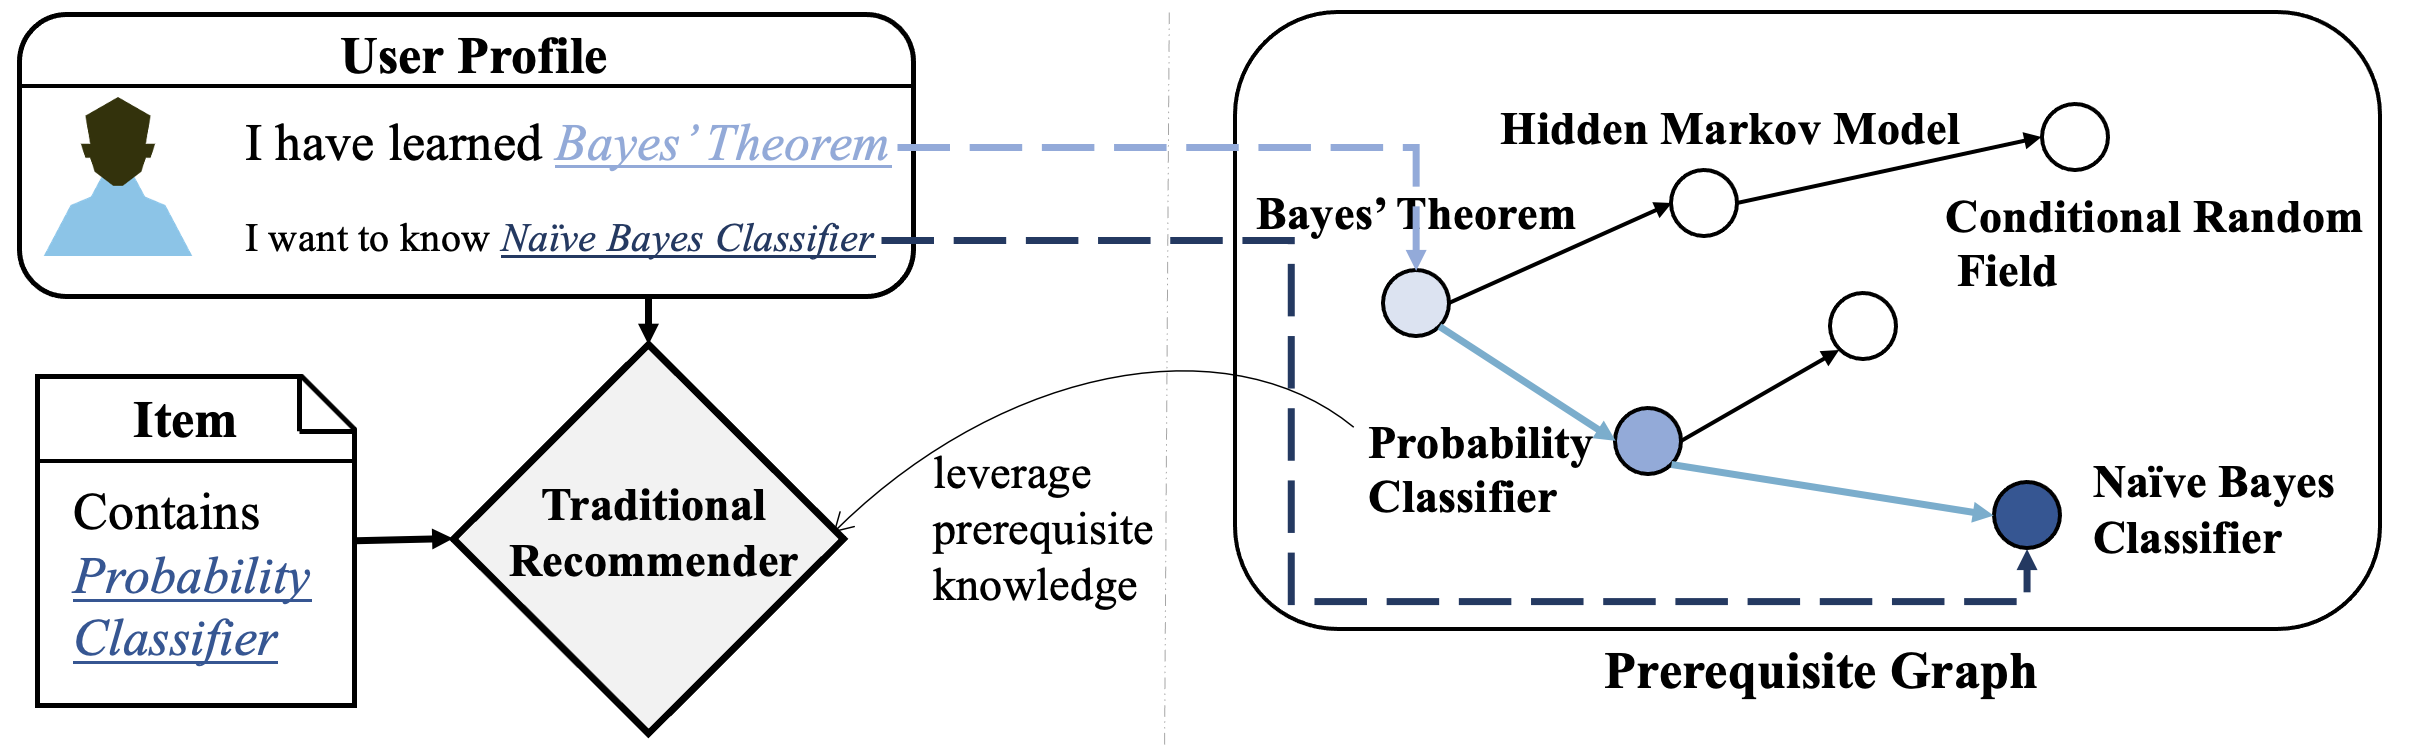
\includegraphics[width=0.7\linewidth]{res/intro_example_hori.png}
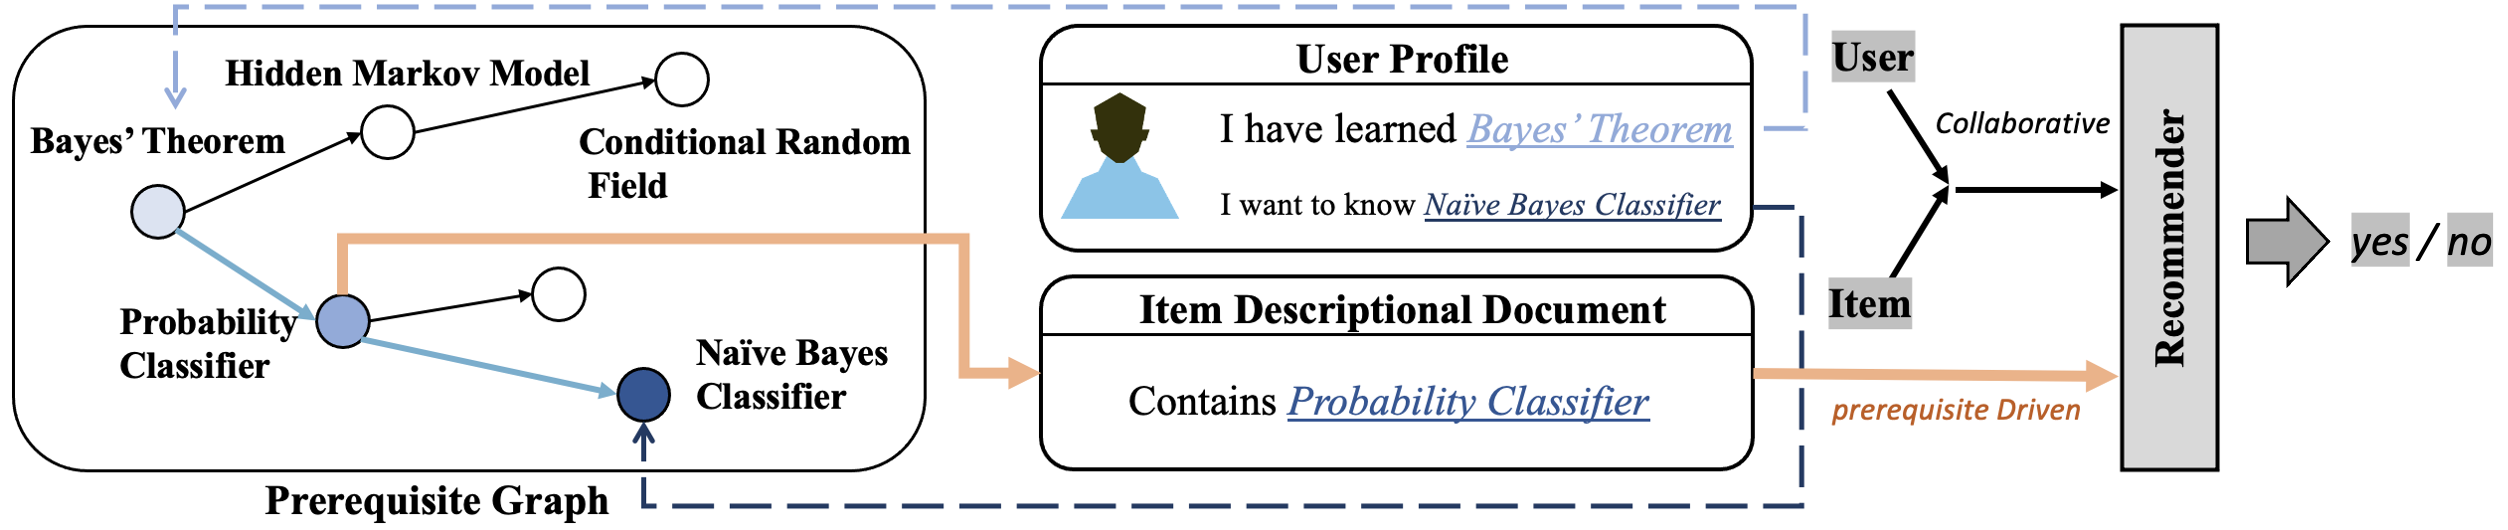
\includegraphics[width=0.88\linewidth]{res/intro_new.png}
\caption{An illustration of prerequisite driven recommendation: in which a recommender (right) incorporates prerequisite knowledge (left), distilled from both user and item prerequisite context.
Dashed edges link users to the concepts they have mastered as prior concepts and the desired concepts to acquire as target knowledge. }
\label{fig:example}
\end{figure}

% Method
To demonstrate the effectiveness of leveraging prerequisite context for recommendation, we propose a Prerequisite-Driven Recommendation System (PDRS) embodying this  formalism. 
%coupling it to traditional collaborative mechanisms. 
The key challenge here is how to accurately acquire user- and item- forms of prerequisite context for use in recommendation. 
% inferred from the user--item interaction matrix
However, there is an important shortcoming.  Explicit prerequisite knowledge is often sparse, requiring laborious effort to compile.  It is often also brittle, as items and their relationships with underlying contextual concepts can evolve over time.  
Assuming manually-labeled prerequisites \cite{vuong2011method,talukdar2012crowdsourced} is often unrealistic due to the heavy cost of human annotation.  An automatic means of inferring prerequisites is called for.
% Holden: @Min. Need double-check below.
% MinCR: proofread looks good.
We address this in two parts by contributing a) an automatic key knowledge concept extractor from item descriptive text, and b) a prerequisite relation constructor for concept pairs by inferring prerequisite weights from both internal and external domain features.
Our encoding components finds a suitable representation of a user in terms of prior and target knowledge, leveraging pretrained language models. We then integrate such prerequisite context into the recommendation process by joint training of both the recommendation and prerequisite knowledge learning tasks.
% as well as users' prior and target knowledge. 
% Our Prerequisite Context Modeling component constructs users' prior and target knowledge ...
% The prerequisite context leverage the knowledge from side prerequisite knowledge (in the form of topologically-sorted prerequisite graph) 

We evaluate our PDRS system on three datasets representing different domains. We find that PDRS achieves performance gains in recommendation not only in domains where prerequisites exist as hard constraints --- such as (educational) course recommendation --- but also in domains where prerequisites are soft, personal preferences, as in movie and book recommendation. Importantly, we also show that such model makes an especially strong impact in sparse data cold-start scenarios, a pervasive problem in RS. 

% We summarise our contributions as follows: 
% \begin{itemize}
%     \item To the best of our knowledge, we are the first to explore the use of prerequisite context for recommendation.
%     % \item We formalise the framework of prerequisite-driven recommendation consisting three components: 1) the users' prerequisite context and 2) the items' prerequisite context, and 3) the prerequisite graph;
%     \item We instantiate our formalism in the form of a Prerequisite Driven Recommendation System (PDRS; \S~4) embodied as a modern neural architecture, which adopts joint training to optimise the model for the twin objectives of knowledge linking prediction and recommendation;
%     \item We demonstrate that prerequisite context is a functional booster solving cold-start problem, and can benefit recommenders universally through our extensive experiments on our Course, Movie, and Book datasets (\S~5).
% \end{itemize}

